\chapter{Valuation of a Firm}

\section{Introduction}
\begin{itemize}
    \item Recap of the previous session on the dividend discount model (DDM):
      \begin{itemize}
        \item We valued shares based on present value of expected dividends.
        \item We discussed its applicability for mature companies with consistent dividend payouts.
        \item Noted limitations due to the variable nature of dividends.
      \end{itemize}
    \item Introduction to the Discounted Cash Flow (DCF) method:
      \begin{itemize}
        \item Popular among equity research analysts for its flexibility.
        \item Allows for detailed company analysis including scenario testing.
      \end{itemize}
  \end{itemize}

\section{Estimating enterprise value}
A DCF calculates projected future cash flows from company. Projection can be done based on historical data, industry trends, and management forecasts. Next, we must determine the discount rate which is the required rate of return.\\

Discount rate is calculated using weighted average cost of capital (WACC), which takes into account the cost of equity and cost of financing/debt.

Once cash flows and discount rate are determined, the next step is calculating the present value of each projected cash flow (using the discounted rate). The sum of these present values is the enterprise value of the company. Let $r$ be the discount rate, $CF$ be the cash flow, and $n$ be the number of time periods. The present value of cash flow is given by:

\begin{equation}
    PD  = \frac{CF}{(1+r)^n}
\end{equation}

In many cases the projected cash flows extend for a finite period. To account for the value beyond the projected period, a terminal value is used at the end of that period, which assumes a constant growth rate. The terminal value (TV) is calculated as \textbf{Gordon Growth Model}:

\begin{equation}
    TV = \frac{CF_{n+1}}{r-g}
\end{equation}

(There is also an exit multiple method, which uses a multiple of EBITDA or EBIT to calculate terminal value.)

This terminal value is discounted back to its present value using the discount rate. 

Add the present projected value and the present terminal value to get the enterprise value (V).

\begin{equation}
    V = \sum_{i=1}^{n} \frac{CF_i}{(1+r)^i} + \frac{CF_{n+1}}{r-g}
\end{equation}

Calculate the share price or equity value: deduct the net debt from the enterprise value and divide by the number of shares outstanding. Equity value is the firm's value V, minus any liabilities (in our simplified model all liabilities are just debt).

\begin{equation}
    \text{Equity Value } E = \frac{V - \text{Net Debt } D}{\text{Shares Outstanding}}
\end{equation}

Two valuation approaches (DDM) and (DCF) are both used. DDM is problematic when companies have a discretionary dividend policy, or when they have a high growth rate. DCF is more flexible and practical as it can be used for companies with no dividends, or when dividends are not a good indicator of company performance. This is because it incorporates all cash flows to estimate the company's enterprise value.\\

For DCF to work, cash flow estimations must be accurate. \textbf{Assume the company is 100\% equity financed for now.} \\

Focusing on the income statement, note the free cash flow, generated for all capital lenders to the firm (debt and equity). 

\subsection*{EBIT (Earnings Before Interest and Tax)}
\begin{equation}
    EBIT = \text{Revenue} - \text{Operating Expenses}
\end{equation}

Not all cash flows are available to investors, as the company must pay taxes and cover other costs to reinvest into the business. So the free cash flow is calculated as:

\begin{align}
    \text{Total Cash Flow } &= EBIT (1-t) + \text{Depreciation}\\
    \text{Free Cash Flow } &= EBIT (1-t) + \text{Depreciation} - \text{Capital Expenditure} - \text{Change in Net Working Capital (NWC)}\\
    &= \text{Total Cash Flow} - \text{Capital Expenditure} - \text{Change in Net Working Capital (NWC)}
\end{align}

If the company is partially debt-financed, the cost of debt must be accounted for as the company's tax bill is less due to tax exemption on debt. This adjustment is made in the discount rate which is lowered to account for the tax shield. This discount rate is the WACC, or the weighted average cost of capital.\\

A terminal value is calculated at the end of the projection period, similar to the DDM. A constant growth rate is assumed for the terminal value. 

\begin{equation}
    TV = \frac{FCF_{N+1}}{r_{WACC}-g}
\end{equation}

\begin{equation}
    FCF_{N+1} = FCF_N^*(1+g)
\end{equation}

\renewcommand{\thesection}{4.3 - 4.5}
\section{Calculating Enterprise Value}
\setcounter{section}{5}
\renewcommand{\thesection}{\arabic{chapter}.\arabic{section}}

\subsection*{Case Study: Apple}
\begin{itemize}
    \item 2012: Apple's stock was at \$700.
    \item 2014: 7-1 stock split, reducing the price to \$100.
    \item Apple felt the share price was too high, so it was split to improve liquidity
    \item Apple was one of the largest companies by market capitalisation in 2023, with a valuation of nearly \$2.8 trillion.
     \begin{figure}[H]
        \centering
        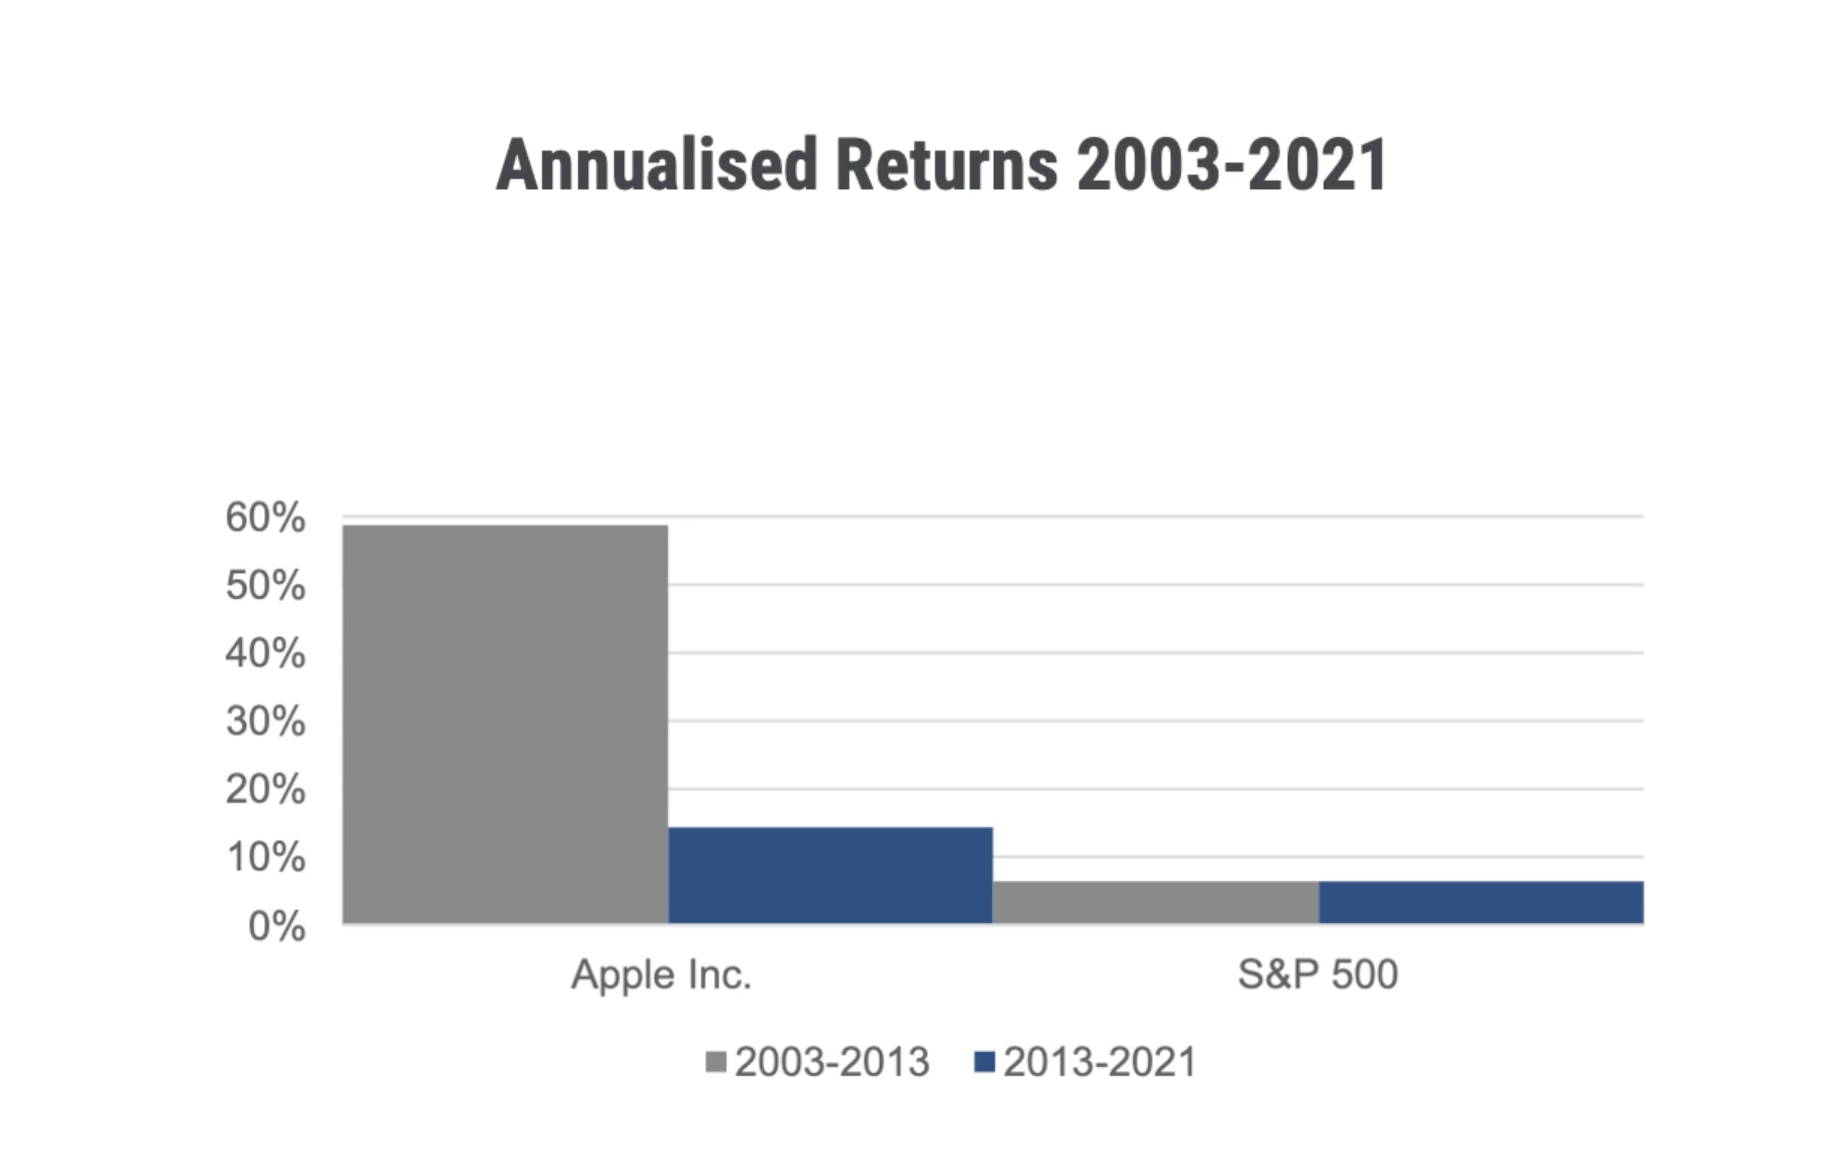
\includegraphics[width=0.5\textwidth]{img/4.3.png}
        \caption{Annualised returns 2003-2021}
    \end{figure}
    \item Apple is a tech giant and its success lies in the synergies of its products.
    \item To best value Apple, we must look at the aggregate level.
     \begin{figure}[H]
        \centering
        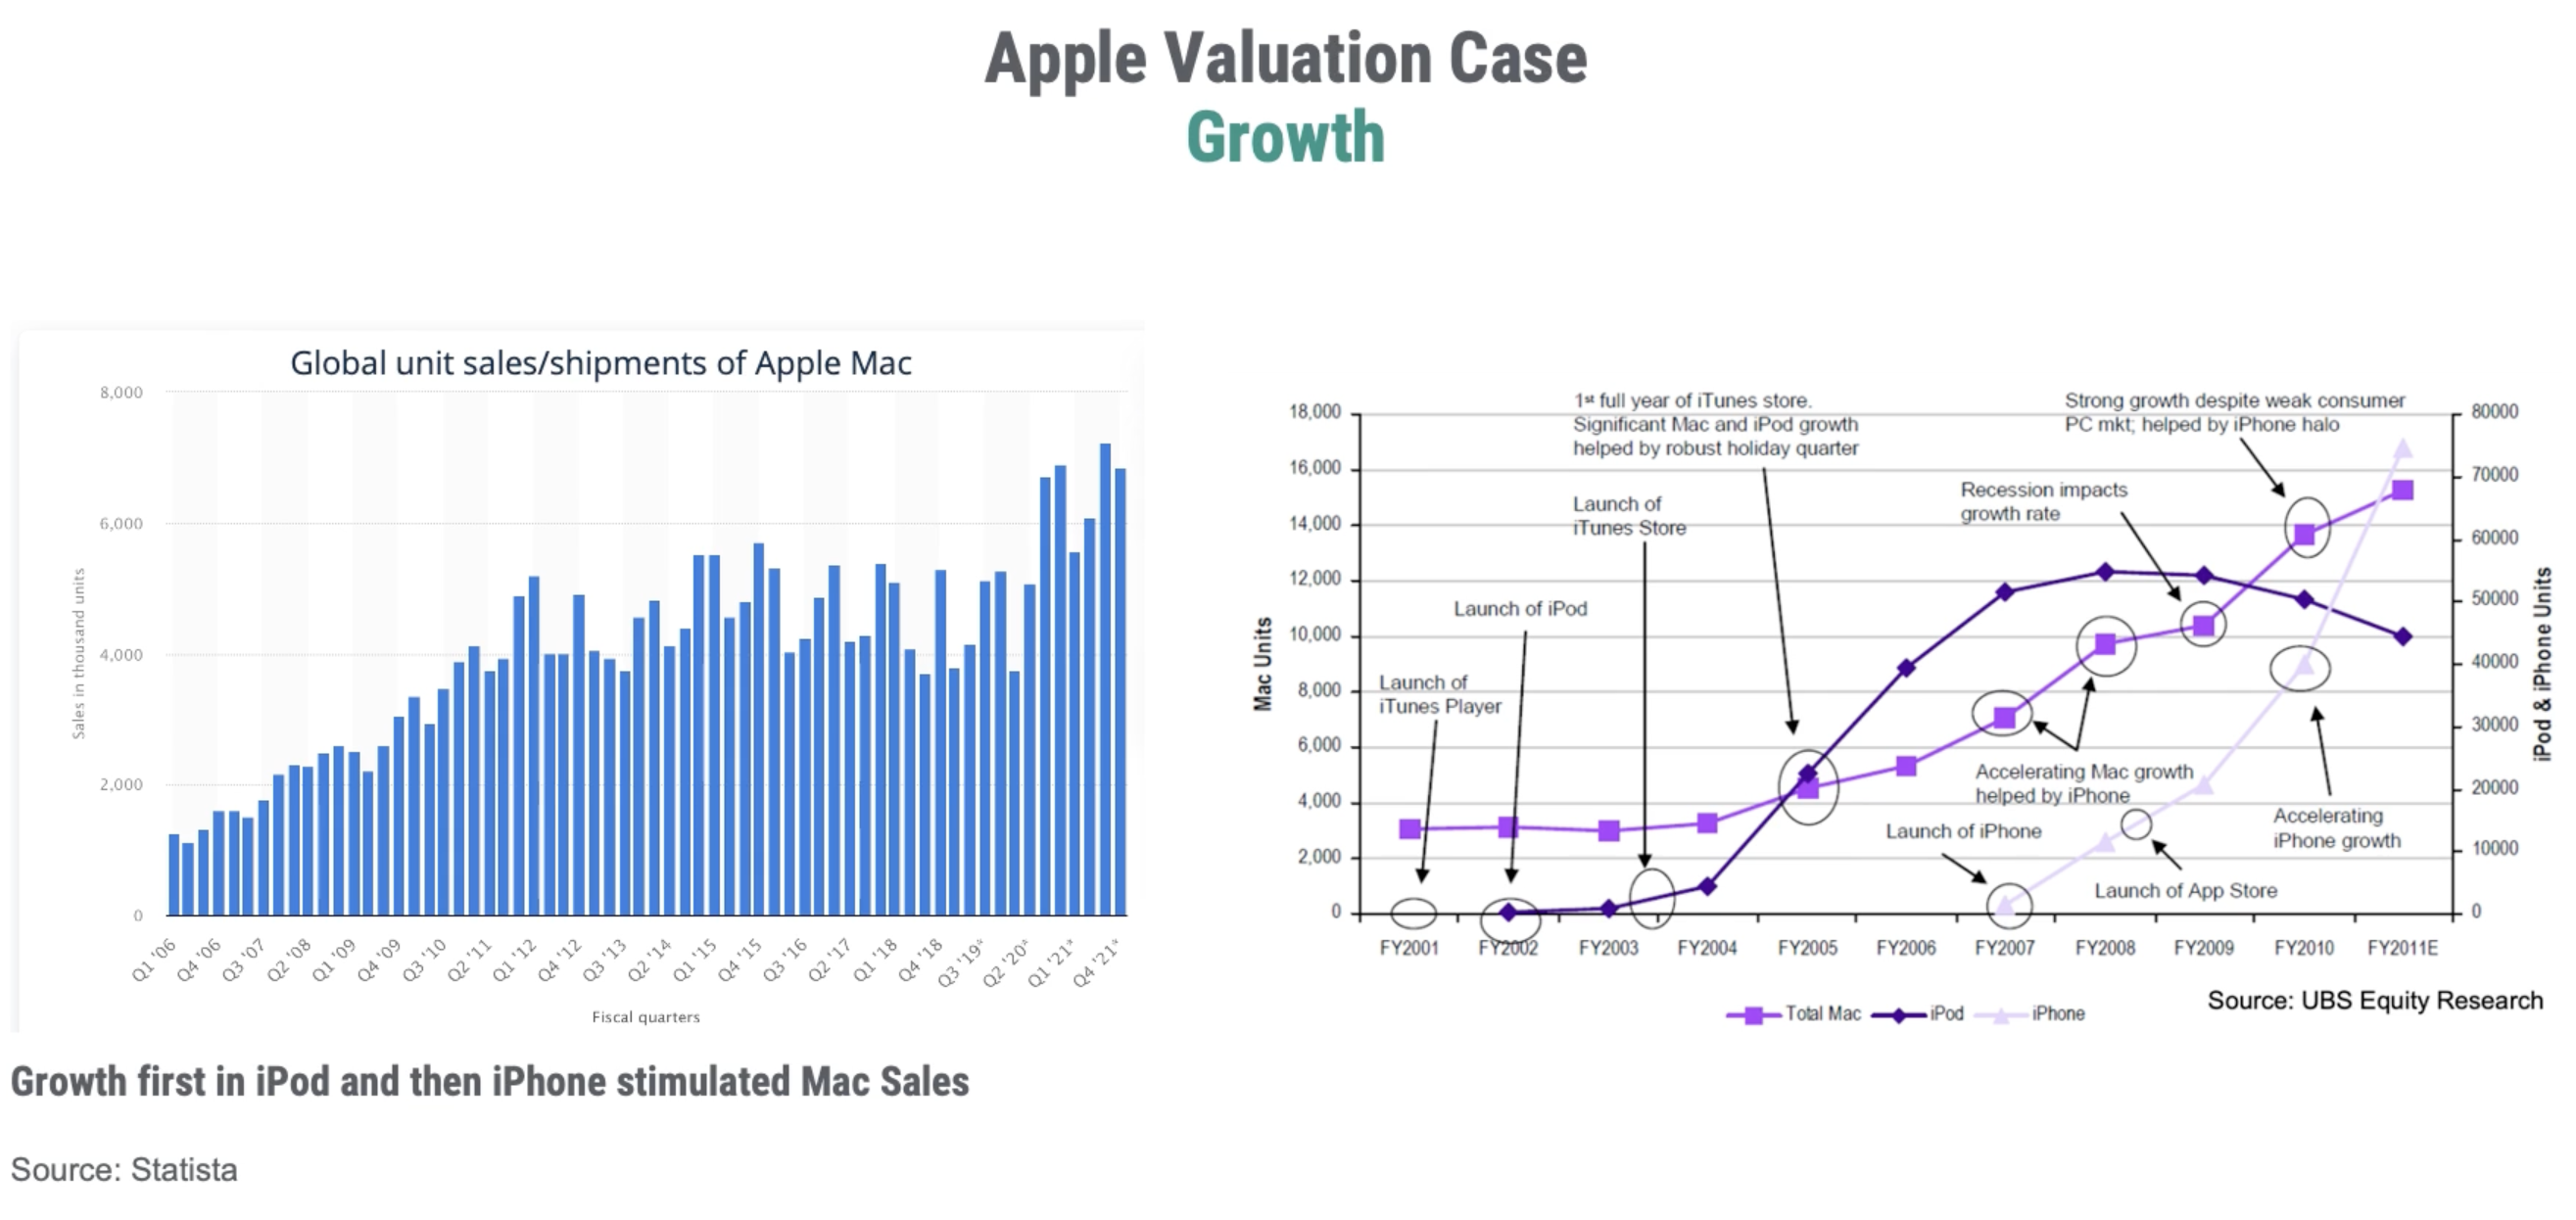
\includegraphics[width=0.5\textwidth]{img/4.4.png}
    \end{figure}
    \begin{figure}[H]
        \centering
        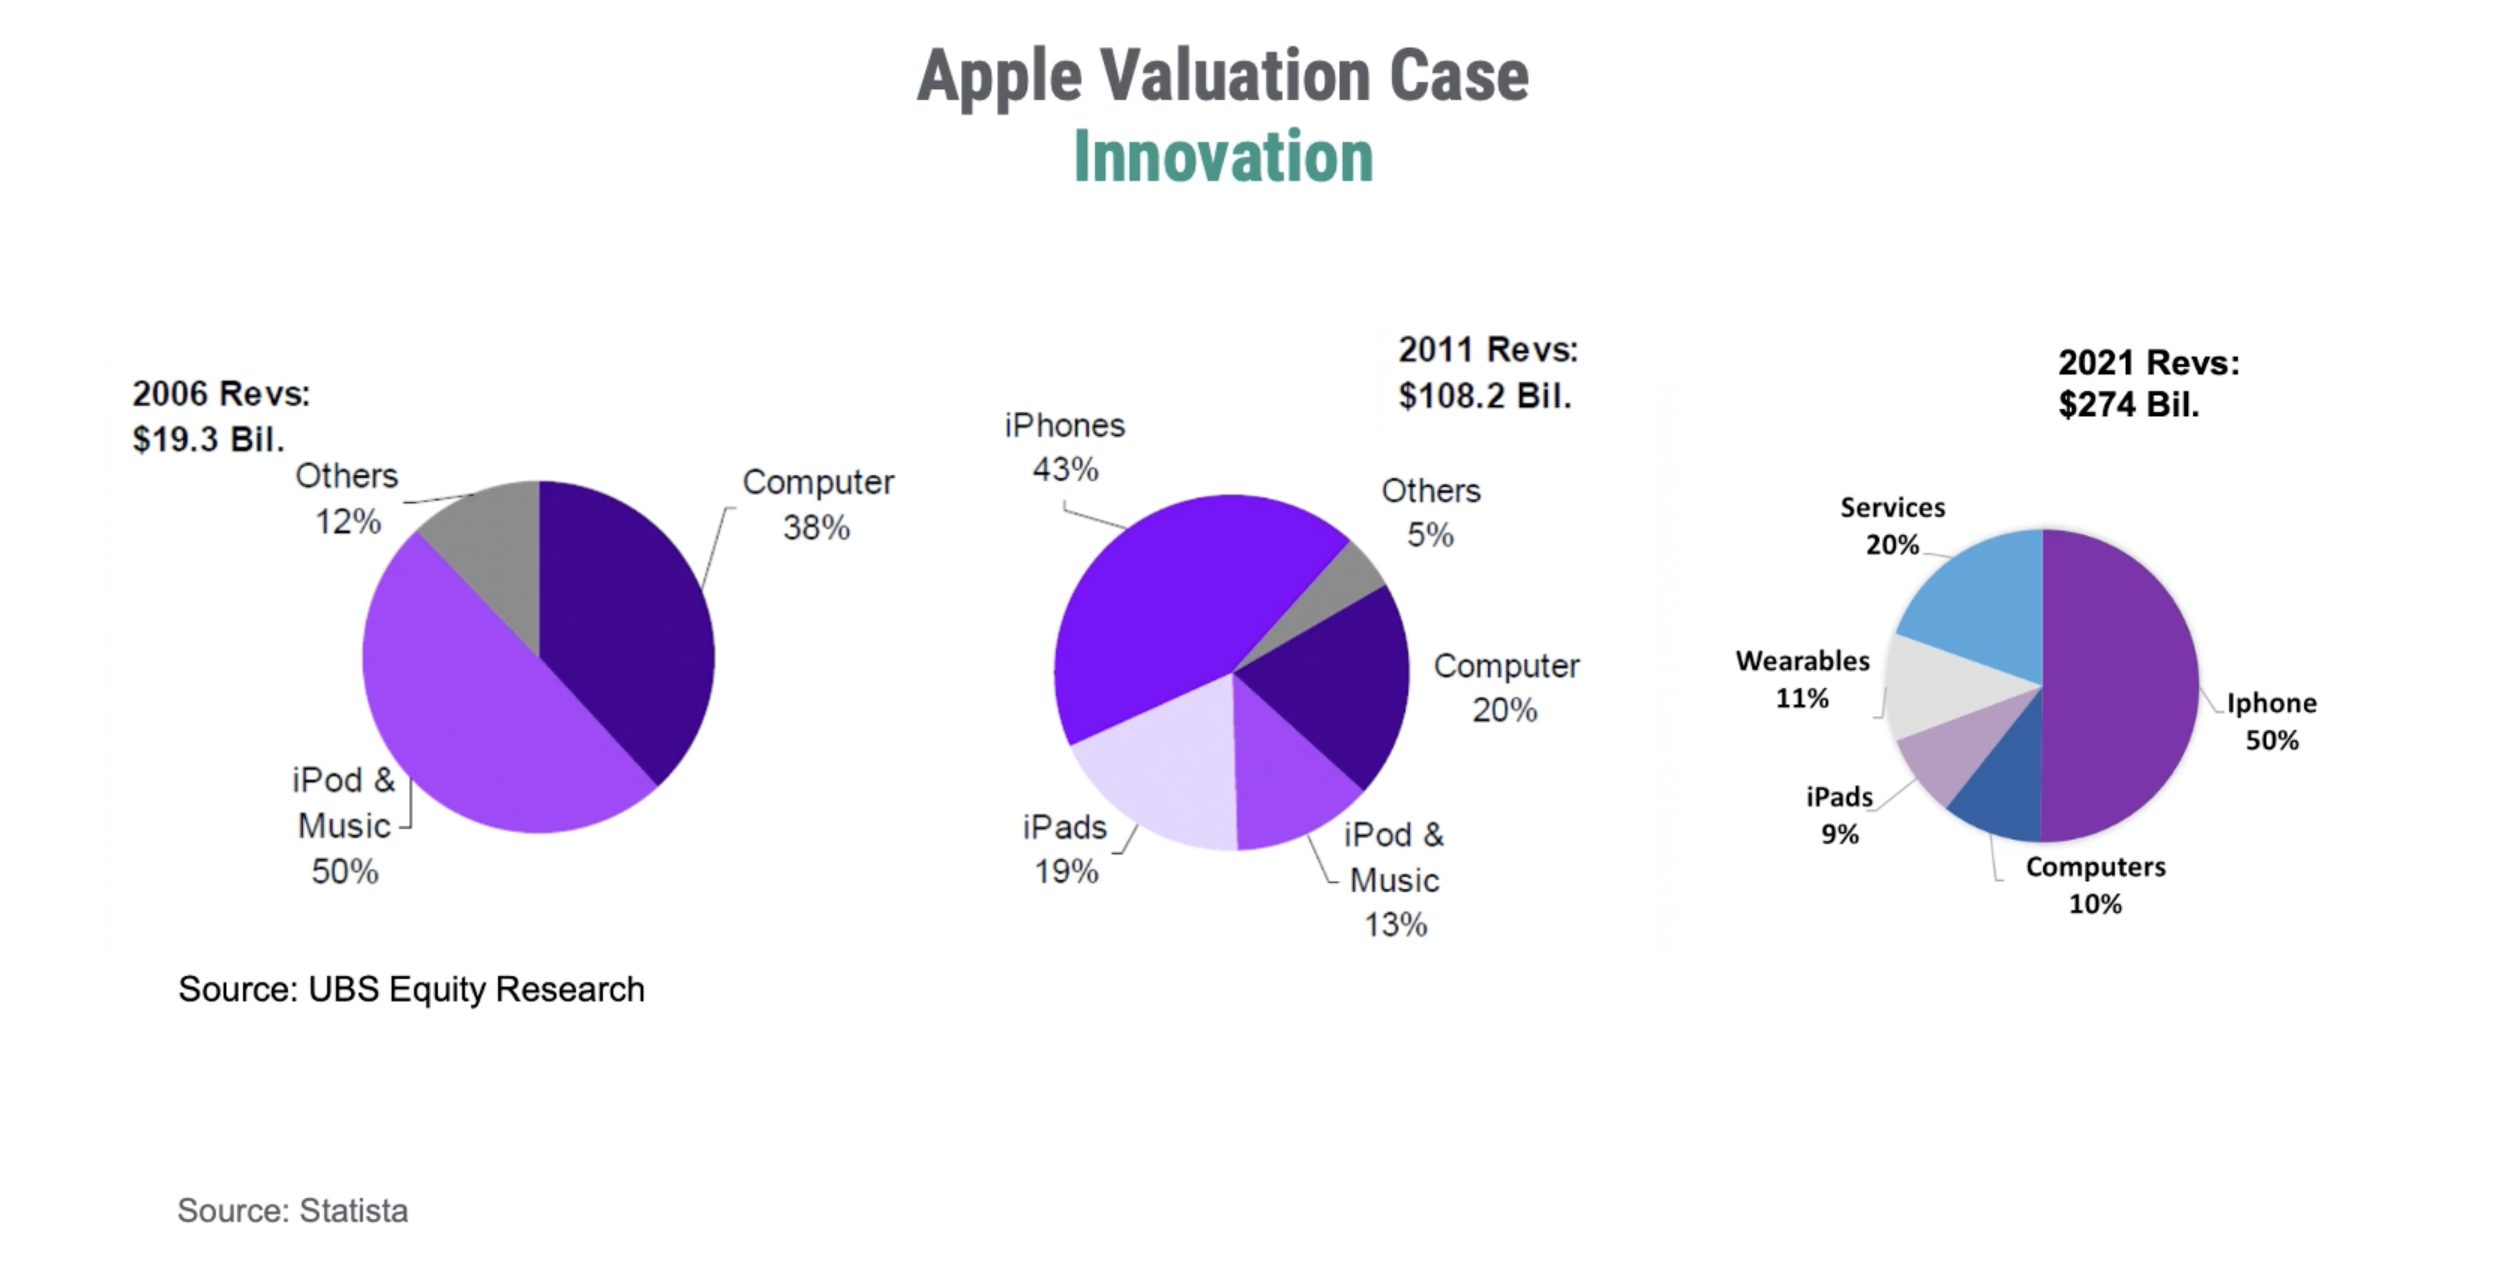
\includegraphics[width=0.5\textwidth]{img/4.5.png}
    \end{figure}
    \item One boost in a product's sales will have a knock-on effect on other products.
    \item It has large profit margins, and a large cash pile.
    \item There have been large return on equity (ROE) and return on assets (ROA) in recent years.
    

\end{itemize}

\begin{table}[ht]
    \centering
    \caption{Apple's Past Performance}
    \label{my-label}
    \tiny
    \begin{tabular}{|l|r|r|r|r|r|r|r|r|r|r|r|}
    \hline
    \textbf{millions of dollars} & \textbf{2012} & \textbf{2013} & \textbf{2014} & \textbf{2015} & \textbf{2016} & \textbf{2017} & \textbf{2018} & \textbf{2019} & \textbf{2020} & \textbf{2021} & \textbf{2022} \\ \hline
    Long term debt               & -             & 16,960        & 28,987        & 53,329        & 75,427        & 97,207        & 93,735        & 91,807        & 98,667        & 109,106       & 148,101       \\ \hline
    Revenue, Total               & 156,508       & 170,910       & 182,795       & 233,715       & 215,639       & 229,234       & 265,595       & 260,174       & 274,515       & 365,817       & 394,328       \\ \hline
    EBIT                         & 55,241        & 48,999        & 52,503        & 71,230        & 60,024        & 61,344        & 70,898        & 63,930        & 66,288        & 108,949       & 119,437       \\ \hline
    Net income                   & 41,733        & 37,037        & 39,510        & 53,394        & 45,687        & 48,351        & 59,531        & 55,256        & 57,411        & 94,680        & 99,803        \\ \hline
    Effective tax rate \%         & 25.2          & 56.2          & 26.1          & 26.4          & 25.6          & 24.6          & 18.3          & 15.9          & 14.4          & 13.3          & 16.4          \\ \hline
    Market capitalisation        & 560,013       & 472,269       & 616,453       & 664,970       & 516,362       & 885,669       & 956,625       & 1,105,307     & 1,850,816     & 2,337,583     & 2,241,050     \\ \hline
    Total dividends paid         & 2,488         & 10,564        & 11,126        & 11,561        & 12,150        & 12,769        & 13,712        & 14,081        & 14,467        & 14,841        & 14,841        \\ \hline
    Repurchase of stock          & 1,226         & 23,942        & 46,158        & 36,752        & 31,292        & 34,774        & 75,265        & 69,714        & 92,527        & 89,402        & -             \\ \hline
    Payout ratio                 & 6.0           & 28.5          & 28.2          & 21.7          & 26.6          & 26.4          & 23.0          & 25.6          & 15.3          & 14.9          & -             \\ \hline
    Total payout ratio           & 8.9           & 93.2          & 145.0         & 90.5          & 95.1          & 98.3          & 149.5         & 151.7         & 113.0         & 104.4         & -             \\ \hline
    Operating margin \%   & 35.3          & 28.7          & 28.7          & 30.5          & 27.8          & 26.8          & 26.7          & 24.6          & 24.1          & 29.8          & 30.3          \\ \hline
Effective tax rate    & 25.2          & 56.2          & 26.1          & 26.4          & 25.6          & 24.6          & 18.3          & 15.9          & 14.4          & 13.3          & 16.4          \\ \hline
CAPX + R\&D rate      & 7.5           & 7.4           & 8.5           & 8.3           & 10.6          & 10.5          & 10.4          & 10.3          & 9.5           & 9.0           & 9.4           \\ \hline
Return on Equity \% (ROE) & 42.8       & 30.6          & 33.6          & 46.2          & 36.9          & 36.9          & 49.4          & 60.9          & 87.9          & \textbf{150.1  }       & \textbf{158.2}         \\ \hline
Return on Assets \% (ROA) & 23.6       & 16.0          & 15.0          & 17.1          & 12.3          & 11.0          & 12.0          & 18.9          & 20.5          & \textbf{31.0}          & \textbf{34.0}          \\ \hline
    \end{tabular}
    \normalsize % Resets the font size to normal for the rest of the text.
    \end{table}
    

Let's determine if Apple is overvalued or undervalued. 

\begin{itemize}
    \item Use average analyst consensus forecasts for the future years 2023-2024 from Reuters
    \item Use analyst forecasts of capital expenditure assume it to grow in line with revenues after 2023
    \item From 2025-2028, assume 6\% growth rate aligning with GDP
    \item 2029 and beyond, a more conservative 4\% growth rate
    \item Assume constant margins of just under 30\%
    \item Assume constant tax rates at 16.5\% of EBIT
    \item Use to calculate free cash flows from 2023-2028
    \item Networking capital investment is assumed to be proportional to revenue
\end{itemize}

Terminal value is estimated using a present value formula, with a discount rate WACC of 10.5\% and a perpetual growth rate of 4\%.

\begin{align}
    TV = \frac{FCF_{2028}}{r_{WACC}-g}\\
    FCF_{2028} = FCF_{2027}*(1+g)
\end{align}

\begin{table}[ht]
    \centering
    \caption{Financial Overview}
    \label{table:financial_overview}
    \small
    \begin{tabular}{|l|r|r|r|r|r|r|r|}
    \hline
    \textbf{}                 & \textbf{2022}     & \textbf{2023}     & \textbf{2024}     & \textbf{2025}     & \textbf{2026}     & \textbf{2027}     & \textbf{2028}     \\ \hline
    Revenue growth rate \%    & -                 & 6.0               & 5.9               & 5.0               & 5.0               & 5.0               & 5.0               \\ \hline
    Earnings growth rate \%   & 9.63\%            & 8.9               & 5.9               & 5.0               & -                 & -                 & -                 \\ \hline
    Revenues                  & 394,328           & 417,988           & 442,649           & 464,781           & 488,020           & 512,421           & 538,043           \\ \hline
    Operating Margin          & 30.3              & 0.31              & 0.28              & 0.30              & 0.30              & 0.30              & 0.30              \\ \hline
    Operating Income (EBIT)   & 119,437           & 130,082           & 137,746           & 139,434           & 146,406           & 153,726           & 161,413           \\ \hline
    Effective tax rate \%     & 13.3              & 17,301            & 18,320            & 18,545            & 19,472            & 20,446            & 21,468            \\ \hline
    NOPAT                     & 103,551.88        & 112,781           & 119,426           & 120,890           & 126,934           & 133,281           & 139,945           \\ \hline
    Depreciation              & 11,104            & 10,780            & 11,899            & 12,494            & 13,119            & 13,775            & 14,464            \\ \hline
    CAPX                      & 10,708            & 10,396            & 11,475            & 12,049            & 12,651            & 13,284            & 13,948            \\ \hline
    Change in NWC             & (27,932)          & (29,607.92)       & (31,354.79)       & (32,922.53)       & (34,568.65)       & (36,297.09)       & (38,111.94)       \\ \hline
    Free Cash Flow (FCF)      & 131,880           & 142,773           & 151,205           & 154,258           & 161,971           & 170,069           & 178,573           \\ \hline
    \end{tabular}
    \normalsize % Resets the font size to normal for the rest of the text.
    \end{table}

    \begin{table}[ht]
        \centering
        \caption{Valuation Summary}
        \label{table:valuation_summary}
        \begin{tabular}{|l|r|}
        \hline
        \textbf{Item}                 & \textbf{Value} ('000s)    \\
        \hline
        EV (sum of PV FCF)            & 2,706,512         \\
        \hline
        Net debt                      & 84,129            \\
        \hline
        Equity                        & 2,622,383         \\
        \hline
        \#Shares Outstanding          & 15,787            \\
        \hline
        Share price                   & 166.11            \\
        \hline
        \end{tabular}
    \end{table}
        

\begin{itemize}
    \item Discounting all the cash flows back to 2022, we get the estimated enterprise value of Apple which is \$2.7 trillion. 
    \item Subtracting net debt of \$84 billion, we get \$2.6 trillion of equity value. 
    \item Divide this by the number of shares outstanding, we get a share price of \$166.11
    \item The DCF is very close to the actual market capitalisation of Apple. This shows that the DCF model is a good way to value companies.
    \item The share price at the end of 2022 was actually \$130, so Apple was undervalued.
    \item These estimates are sensitive as they are based on assumed growth rates
    \item Apple's case illustrates the impact of volatile operating conditions paired with strong cash flow and balance sheet management on share buybacks.
    \item In May 2018, Apple initiated a \$100 billion share repurchase program, significantly increasing their history of substantial buybacks since 2013, influenced by the activist investor Carl Icahn.
    \item By August 2018, Apple's share price hit a record peak. However, on January 4, 2019, amidst heightened market volatility, especially in tech stocks, Apple's shares saw their largest drop since 2013, nearly 10\%, following a forecast of lower quarterly sales largely due to iPhone sales.
    \item Despite these challenges, Apple's business model transformation since 2019 has been fruitful, with the stock yielding annual returns exceeding 25\% from 2019 to 2023.
  \end{itemize}

\section{Comparables}

The \textbf{multiples} or \textbf{comparables} method is another simpler way to value a company. It involves comparing the company to similar companies in the same industry. So we assess whether the company is fairly valued in comparison to others. We compare a valuation ratio or multiple of one company to another, and then assess if the company is fairly valued based on this ratio.\\

While multiples are not as accurate as DCF, they provide a rough indication. Relative value investors use this method to identify undervalued companies.\\

The most used multiple is the price-to-earnings (P/E) ratio. This is the share price divided by the earnings per share. A high P/E ratio shows how much investors are willing to pay for each dollar of earnings. A high P/E ratio
indicates that investors expect higher earnings growth in the future.\\

\begin{equation}
    \text{Basic }P/E = \frac{\text{Share Price}}{\text{Earnings per Share}}
\end{equation}

Analysts use different kinds of ratios.\\

There are trailing earnings, which are the earnings of the past 12 months. There are also forward earnings, which are the estimated earnings for the next 12 months. Sometimes an average of the two are used.\\

The typical consensus is to use the 12-month forward PE ratio.

\begin{equation}
    P/E = \frac{\text{Best estimate of current share price}}{\text{Best estimate of earnings per share expected over 12 months}}
\end{equation}

\begin{itemize}
    \item Calculate the forward P/E ratio for each company in your peer group
    \item Calculate the average P/E ratio for the peer group, this is the industry P/E multiple
    \item Analyse the target company's P/E ratio and compare it to the industry average.
    \item If it is higher, then it is trading at the higher multiple (relatively more expensive than peers)
    \item If it is lower, then it is trading at a lower multiple (relatively cheaper than peers)
    \item A fair value can be estimated by multiplying the industry P/E ration by the earnings per share of the company in question.

\end{itemize}

\begin{equation}
    \text{Fair Value (of the share)} = \text{Industry P/E ratio} \times \text{Earnings per Share of Target Company}
\end{equation}

This is a relatively straightforward model but has its limitations. Its simplicity means it does not account for differences between companies' practices. When a company trades at a different multiple than its peers, it is important to investigate if there are valid reasons for this behaviour.\\

Consider the \textbf{capital structure} of the company such as its equity-to-debt ratio, which can affect the P/E ratio. A company with a higher debt ratio will have a lower P/E ratio.\\

If you have identified an opportunity, use multiple ratios to confirm your findings, e.g. price-to-sales, enterprise-value-to-earnings, price-to-book, etc. Some multiples are more suited for some industries e.g. enterprise-value-to-number-of-subscribers for tech companies.

\section{DCF and pro-forma financial statements}
\href{https://youtu.be/ynlAcc99b4c}{Video link}

\begin{itemize}
    \item A pro-forma is a financial statement that is based on assumptions and projections. It is used to estimate the future financial performance of a company.
    \item It essentially forecasts the next years' performances, up to the terminal value.
    \item The terminal value is the estimated sale price of the company at the final period in the pro-forma.
    \item Take the final sales value, multiply to infer earnings, divide by (r-g) to get the terminal value.
    \item $r$ is usually the interest rate + a few percentage points (risk premium)
    \item Take sales, multiply by sales profitability to get earnings, discount it back
    \item Generally, it's very hard to come up with an accurate pro-forma, let alone predict the future.
\end{itemize}

To summarise, once we have completed the assumptions, we are able to work out the present value of forecasted cash flows. When adding in the terminal value, we can calculate the enterprise value. Subtracting the net debt, we can calculate the equity value. Dividing this by the number of shares outstanding, we can calculate the share price. In our example, we believe the share price is overvalued by 32.35\%.

